\documentclass[tikz,border=10pt]{standalone}
% no extra libraries needed
\begin{document}
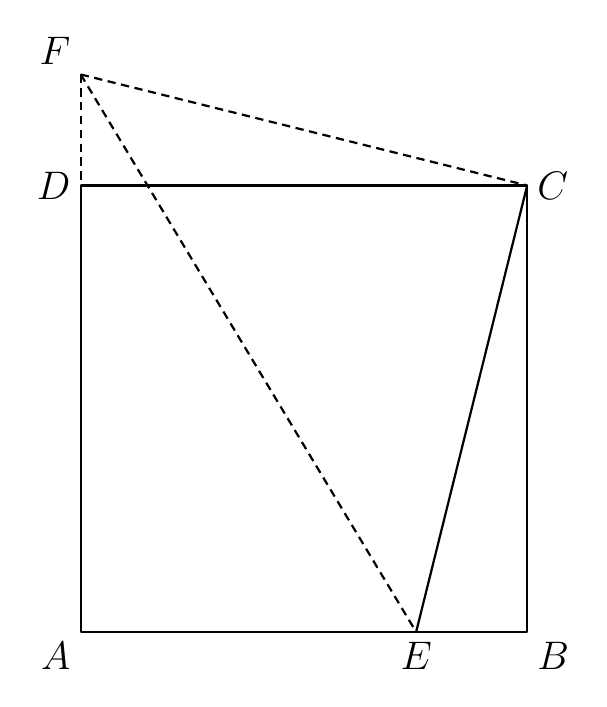
\begin{tikzpicture}[line join=round, line width=0.8pt]
  % Named coordinates (1 unit = 100 px, origin at A, y up)
  \coordinate (A) at (0,0);
  \coordinate (B) at (5.67,0);
  \coordinate (C) at (5.67,5.67);
  \coordinate (D) at (0,5.67);
  \coordinate (E) at (4.26,0);
  \coordinate (F) at (0,7.08);

  % Solid square ABCD
  \draw (A) -- (B) -- (C) -- (D) -- cycle;

  % Solid segment EC
  \draw (E) -- (C);

  % Dashed segments FD, FC, FE
  \draw[dash pattern=on 3pt off 2pt] (F) -- (D);
  \draw[dash pattern=on 3pt off 2pt] (F) -- (C);
  \draw[dash pattern=on 3pt off 2pt] (F) -- (E);

  % Labels enlarged to \Large (positions unchanged)
  \node[below left]  at (A) {\Large $A$};
  \node[below right] at (B) {\Large $B$};
  \node[right]       at (C) {\Large $C$};
  \node[left]        at (D) {\Large $D$};
  \node[below]       at (E) {\Large $E$};
  \node[above left]  at (F) {\Large $F$};
\end{tikzpicture}
\end{document}